\documentclass{article}
\usepackage{graphicx}
\usepackage{fancyhdr}
\pagestyle{fancy}
\lhead{Ruicheng Wu}
\rhead{07/29/2017}
\chead{Homework 12}

\begin{document}
1.
a) lack:
reflexive property

b) it is a partial order

c) lack:
antisymmetric property,because we have both $a \leq b$ , $b \leq a$,
which should implies $a = b$

d) lack:
transitive property,need $a \leq c$

2.(All graph shows in order of Hasse diagram, comparability graph and
incomparability graph)

a)

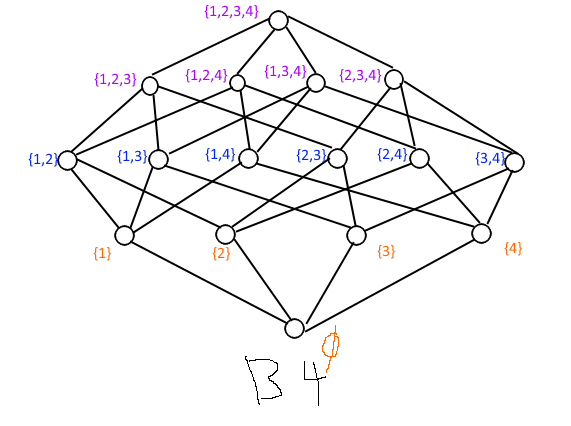
\includegraphics[scale=0.6]{HW12_2a.png}

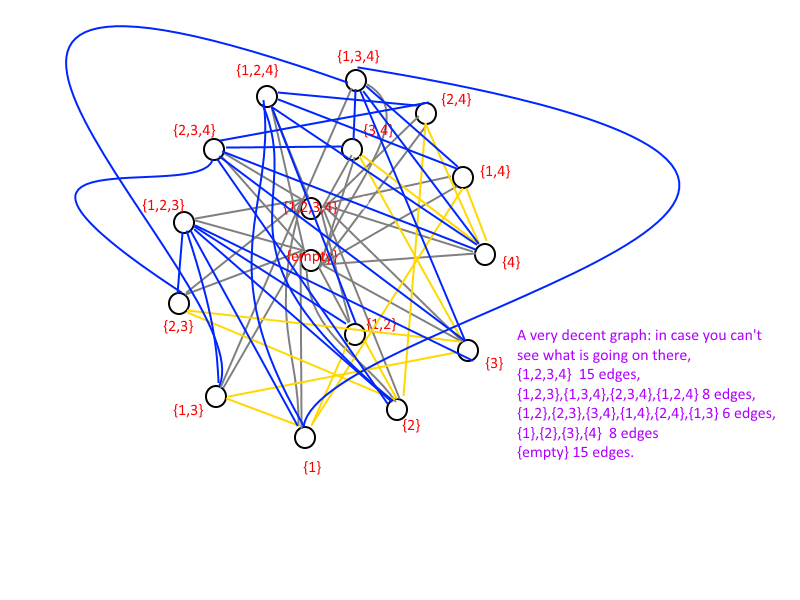
\includegraphics[scale=0.5]{HW12_2a2.png}

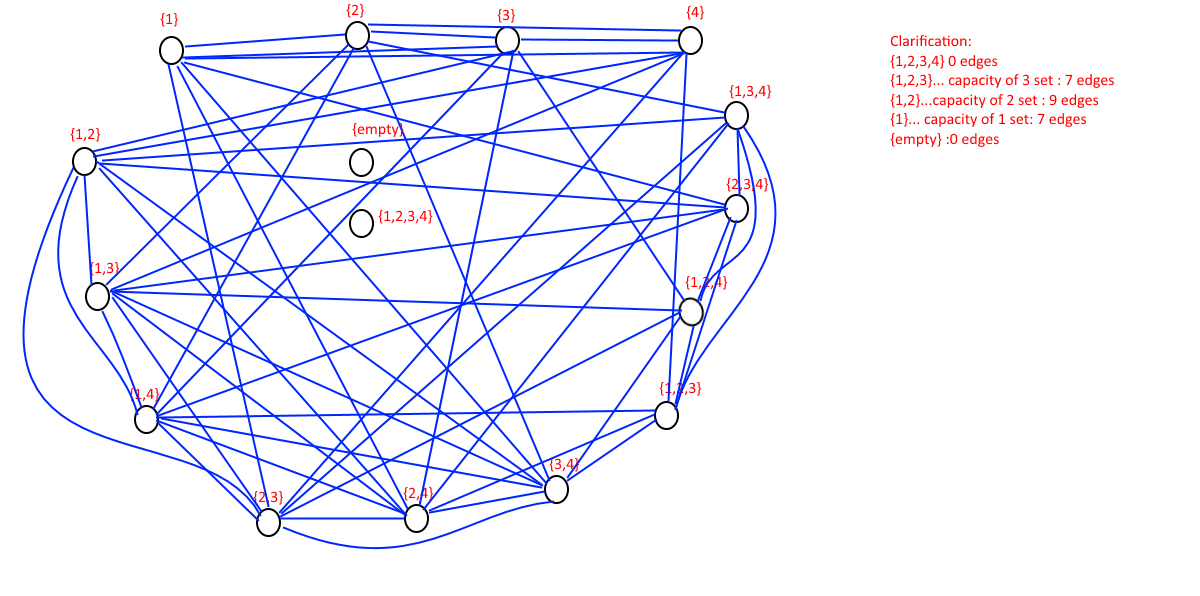
\includegraphics[scale=0.5]{HW12_2a3.png}

b)

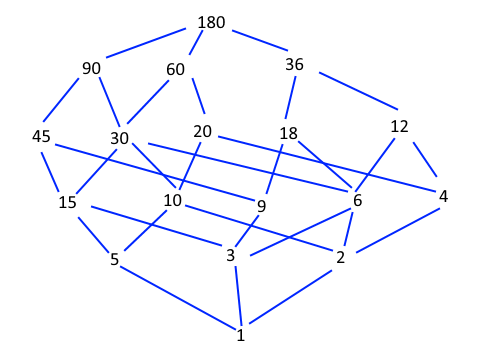
\includegraphics[scale=0.4]{HW12_2b.png}

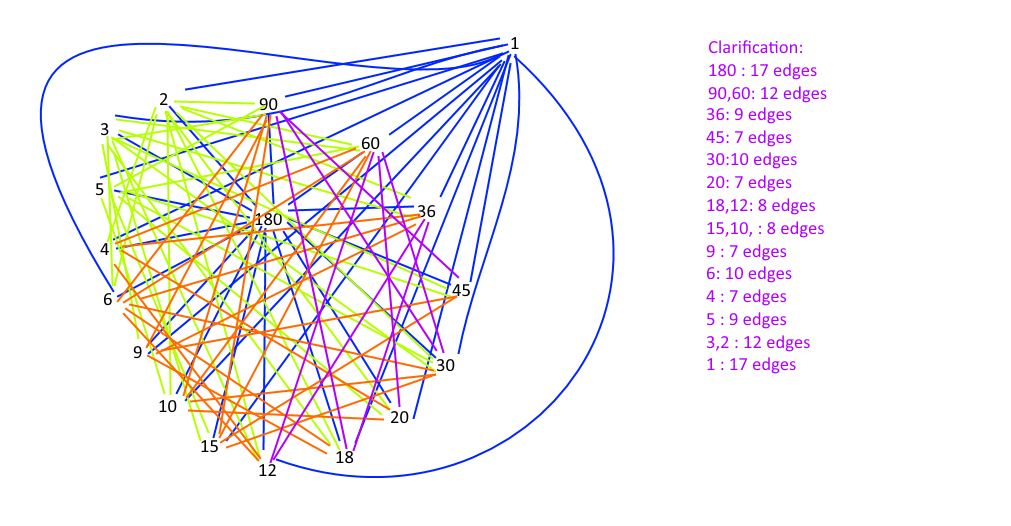
\includegraphics[scale=0.6]{HW12_2b2.png}

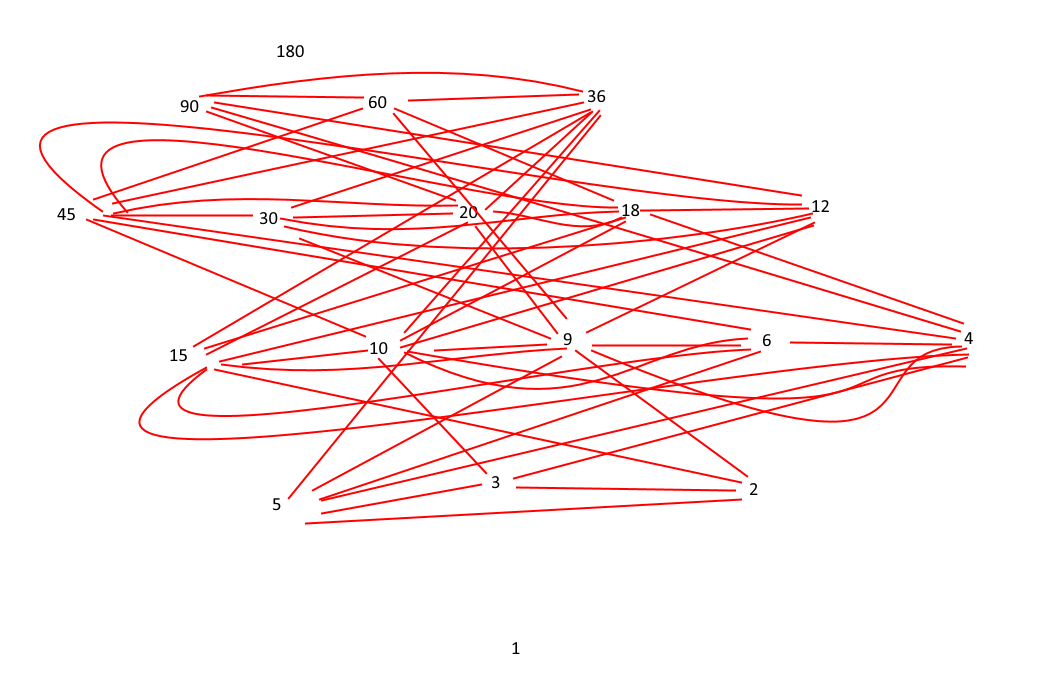
\includegraphics[scale=0.4]{HW12_2b3.png}

c)

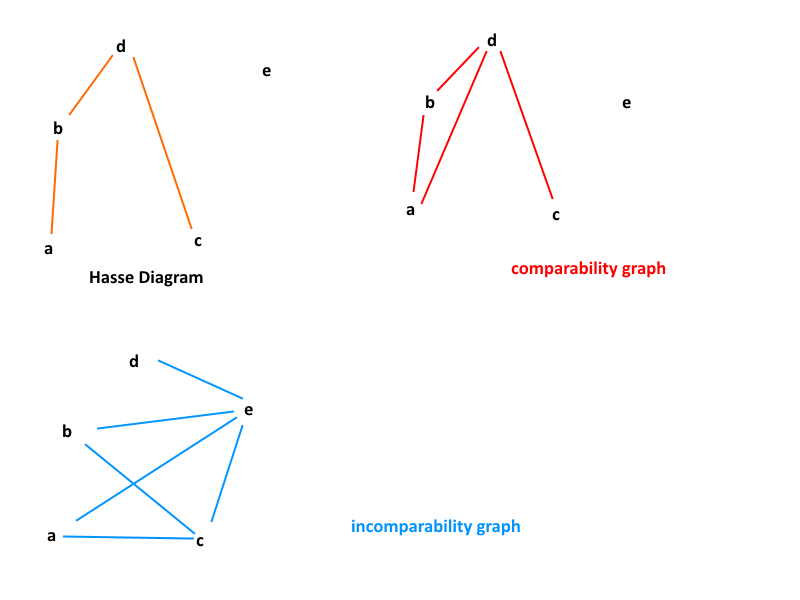
\includegraphics[scale=0.6]{HW12_3.png}

3.

a){1,2,3,4,7,8,17}

b){10,14,15,16,18}

c)height is 5, if you follow (4,5,6,9,14)

d)
According to Dilworth’s Theorem : It is possible to decompose a finite poset P into
width(P), and no fewer, chains.

width(P) = the largest antichains

and we know "Fact 2.0.1. max(P) and min(P) are both antichains."

In our case, it is the |min| = 7.

So we claim it can be partitioned by 7 chains and no fewer.

e)

As said in d), 7.

4.

a)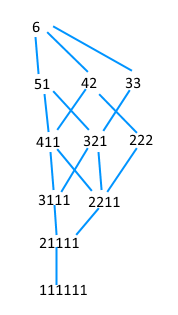
\includegraphics[scale=0.5]{HW12_4.png}

b)

6 , from bottom to top by any path

c)

6, according to Anti-Dilworth’s Theorem: It is possible to decompose a finite poset P into height(P),and no fewer, antichains.And we know the height is the longest chain,in this case is 6.

d)

3,the antichains is in the middle of this lattice. (411,321,222) , (51,42,33)

e)

According to Dilworth’s Theorem : It is possible to decompose a finite poset P into
width(P), and no fewer, chains.

width(P) = the largest antichains

and we know "Fact 2.0.1. max(P) and min(P) are both antichains."

In our case, it is the |min| = 6.

So we claim it can be partitioned by 6 chains and no fewer.

5.

This problem barely asks for largest antichain of a Boolean lattice, according to the Sperner’s Theorem,

the largest antichain of $B_n$ is of size :

$$C(n,floor(n/2))$$ 

$$=C(5,floor(5/2))=C(5,2)= 10$$ 

So size of 10 collection is the largest collection ,$C(5,2)= C(5,3)$,so set contains 2 elements and 3 elements:

such collection could be : 

$$(1,2),(1,3),(1,4),(1,5),(2,3),(2,4),(2,5),(3,4),(3,5),(4,5)$$

$$(1,2,3),(1,2,4),(1,2,5),(1,3,4),(1,3,5),(1,4,5),(2,3,4),(2,3,5),(2,4,5),(3,4,5)$$




\end{document}